
\section{EM algorithm \footnote{Gene Katsevich, Kenneth Tay, Stephen Bates, Nikos Ignatiadis, Dan Kluger and M.H.}}
\label{sec:review_EM}

\subsection{Introduction}
For many interesting statistical models, the log-likelihood is not concave and hence difficult to work with. In order to estimate the parameters by maximum likelihood we must turn to algorithms for non-convex optimization, and the EM algorithm is one useful example. EM is particularly appealing for statistical models involving latent variables, because in these models the EM steps can often be formulated analytically and executed quickly.

\subsection{Motivating example in multiple testing}\label{sec:MT}

Let us assume we are conducting $n$ hypothesis tests based on Z-scores $X_i$. If $i$ is a null hypothesis, then $X_i \sim \nn\p{0,1}$. However, there will also be some $i$'s corresponding to alternatives. A simple model, and a good starting point, to model the alternative distribution is to posit that $X_i \sim \nn\p{\mu,1}$, where $\mu$ depends on the signal strength\footnote{For some applications, it may be better to model the alternative distributions in a non-parametric way}. Of course, we don't know which hypothesis is null or not, so we observe $X_i$ from the mixture distribution:
$$ X_i \sim \pi_0 \mathcal{N}(0,1) + (1-\pi_0)\mathcal{N}(\mu, 1)$$
Here $\pi_0$ is the proportion of null hypotheses. Our goal is to estimate the model parameters, i.e. $\theta = (\mu, \pi_0)$. We can try the maximum likelihood approach. Note that the log-likelihood is
\[ \ell (\theta; X) = \sum_{i=1}^n \log \left( \pi_0 \cdot \phi_0(X_i) + (1 - \pi_0) \phi_{\mu}(X_i) \right). \]
Here we write $\phi_{0}(\cdot)$, resp. $\phi_{\mu}(\cdot)$ for the pdf of a $\nn(0,1)$, resp. $\nn(0, \mu)$ random variable.  The mixture aspect of this problem has led to the log of a sum in $\ell(\theta; X)$, which makes find the MLE difficult:
\begin{itemize}
\item There is no closed form for $\hat{\theta}$, so an iterative approach will be necessary, and
\item $\ell(\theta; T)$ is not concave in $\theta$ and hence an algorithm like Newton--Raphson may be unreliable for calculating the MLE $\hat{\theta}$.
\end{itemize}

The EM algorithm is an iterative approach to maximizing a likelihood, designed for the case when there are latent variables (or missing data) in the problem. In our example, the latent variables are indicators $Z_i \in \{0,1\}$ recording whether $X_i$ is a null or alternative observation. 

\subsubsection*{Complete data log-likelihood}
Thus, for each $i = 1, \dots, n$, let $Z_i$ be the random variable such that $Z_i = 0$ means that the $i$-th test corresponds to a null hypothesis, and $Z_i = 1$ mean that $i$-th test corresponds to an alternative. Our model for $(Z_i,X_i)$ is,
\begin{align*}
    Z_i & \simiid \mathrm{Bern}(1-\pi_0)\\
    X_i \mid Z_i = 0 &\simiid \nn(0,1)\\
     X_i \mid Z_i = 1 &\simiid \nn(\mu,1).
\end{align*}
If we could somehow observe every pair $(Z_i,X_i)$, then we could calculate the log-likelihood based on both $Z_i$ and $X_i$. This is called the \emph{complete data log-likelihood}:
\begin{equation}
\label{eqn:cdll}
\ell(\theta; X, Z) = \sum_{i=1}^n  (1-Z_i) \log(\pi_0 \cdot \phi_{0}(X_i)) + Z_i \log((1 - \pi_0) \cdot \phi_{\mu}(X_i))
\end{equation}
This complete data log-likelihood is much more tractable, we no longer have a sum inside a logarithm. Differentiating \eqref{eqn:cdll} gives the MLE for $\theta$,
\[ \widehat{\pi}_0 = \frac{\sum_{i=1}^n (1-Z_i)}{n}, \qquad \hat{\mu} = \frac{\sum_{i=1}^n Z_i X_i}{\sum_{i=1}^n Z_i}. \]

That's very nice, and exactly what we would have expected. Of course, we can't do this because we don't know the $Z_i$ (else we would not have a multiple testing problem to begin with)!

\subsubsection*{Expected complete data log-likelihood}
While we do not have access to $Z_i$, we do have information about $Z_i$ from $X_i$.  In the spirit of an iterative algorithm, let's assume that we have some guess for the parameters $(\hat{\pi_0}^t, \hat{\mu}^t)$. We can then plug in the conditional expectations of the $Z_i$'s under the parameters $(\hat{\pi_0}^t, \hat{\mu}^t)$ into the complete data log-likelihood \eqref{eqn:cdll}. With this in mind, define
\begin{align*}
\omega_i^t &:= \bbE_{\widehat{\pi}_0^k, \hat{\mu}^k} \left[ 1-Z_i \mid X_i \right] \\
&= P_{\widehat{\pi}_0^k, \hat{\mu}^k} \left[ Z_i = 0 \mid X_i \right] \\ 
&= \frac{P_{\widehat{\pi}_0^t, \hat{\mu}^t} \left[  X_i \mid Z_i = 0\right]P_{\widehat{\pi0}^t, \hat{\mu}^t}\left[Z_i = 0\right]}{P_{\widehat{\pi}_0^t, \hat{\mu}^t} \left[  X_i \mid Z_i = 1\right]P_{\widehat{\pi_0}^t, \hat{\mu}^t}\left[Z_i = 1\right]+P_{\widehat{\pi}_0^t, \hat{\mu}^t} \left[  X_i \mid Z_i = 0\right]P_{\widehat{\pi_0}^t, \hat{\mu}^t}\left[Z_i = 0\right] }\\
&= \frac{ \widehat{\pi}_0^t \phi_{0}(X_i)}{(1-\widehat{\pi}_0^t) \phi_{\hat{\mu}^t}(X_i) + \widehat{\pi}_0^t \phi_{0}(X_i)}.
\end{align*}

Here, $\omega_i^t$ is precisely the probability that $X_i$ is drawn from the null distribution given $X_i$ and the parameters $\hat{\pi}_0^t$ and $\hat{\mu}^t$. Now that we have $\omega_i^t$,  we can write down the \textbf{expected complete data log-likelihood} (the so called ``E''-step) as function of $\theta = (\pi,\mu)$.
\begin{align}
\tilde{\ell}(\theta; \hat{\theta}^t) &:= \bbE_{\widehat{\pi}_0^t, \hat{\mu}^t} \left[ \ell(\theta; X, H) \mid X \right] \label{eqn:estep} \\ 
&=\sum_{i=1}^n \bbE_{\widehat{\pi}_0^t, \hat{\mu}^t} \left[ (1-Z_i) \log(\pi_0 \cdot \phi_{0}(X_i)) + Z_i \log((1 - \pi_0) \cdot \phi_{\mu}(X_i))\right]\\ 
&=\sum_{i=1}^n \omega_i^t \log(\pi_0 \cdot \phi_{0}(X_i)) + (1-\omega_i^t) \log((1 - \pi_0) \cdot \phi_{\mu}(X_i)). \nonumber
\end{align}
That is a nice expression! We can easily optimize this to get our next guess for $\pi_0$ and $\mu$ (the ``M''-step):
\begin{equation}\label{eqn:mstep}
\widehat{\pi}_0^{i+1} = \frac{\sum_{i=1}^n \omega_i^t}{n} , \qquad \hat{\mu}^{t+1} = \frac{\sum_{i=1}^n (1-\omega_i^t) X_i}{\sum_{i=1}^n 1-\omega_i^t}.
\end{equation}


This is in essence what the EM algorithm is: \eqref{eqn:estep} is the E (Expectation) step, while \eqref{eqn:mstep} is the M (Maximization) step.


\subsection{EM as a recipe}

Here is a useful recipe for quals questions. Suppose you have a model $p_{\theta}(X,Z)$ where $\theta$ are the parameters you want to estimate, $X$ is your observed data and $Z$ is your unobserved or latent data. To describe the EM algorithm you should do the following,
\begin{enumerate}[start = 0]
    \item \textbf{Latent variables}: If necessary, introduce latent variables to turn your mixture model into a latent variable model.
    \item \textbf{Complete likelihood}: Write out the complete data log-likelihood,
    \[\ell(\theta;X,Z)= \log(p_\theta(X,Z)). \]
    For some models, this step can be quite involved. Remember that you can write terms of the form $\pi_{Z_i}$ as $\prod_{k=1}^K \pi_k^{I(Z_i=k)}$ where $k=1,\ldots,K$ are the possible values of $Z_i$. It can also be helpful to turn the indicator variables $I(Z_i=k)$ into sums $Y_k = \sum_{i=1}^n I(Z_i=k)$. For example, see Question 5 on the 2014 exam (Section \ref{sec:2014 exam}).
    \item \textbf{E-step}: Fix parameters $\hat{\theta}^t$ and compute the conditional expected value of the complete data log-likelihood,
    \[\tilde{\ell}(\theta;\hat{\theta}^t) = \bbE_{\hat{\theta}^t}[\ell(\theta;X,Z)\mid X].  \]
    In the above expectation, $\theta$ and $X$ are both constants, and so you can pull out functions that only depend on $\theta$ and $X$. The main computation will be calculating the distribution of $Z \mid X$. This is often done using Bayes's rule,
    \[P_{\hat{\theta}^t}(Z \mid X)  = \frac{P_{\hat{\theta}^t}(X \mid Z)P_{\hat{\theta}^t}(Z)}{\int_{X'}P_{\hat{\theta}^t}(X' \mid Z)P_{\hat{\theta}^t}(X')}. \]
    In particular, if $(X,Z) = (X_i,Z_i)$ are i.i.d. pairs and $Z$ is discrete, then it can be helpful to introduce some new notation, 
    \[\omega_{i,k}^t = P_{\hat{\theta}^t}(Z_i=k|X_i), \]
    where $k$ ranges over the possible values of $Z_i$. If $Z$ is not discrete, then you can still use Bayes rule to identify the distribution of $Z|X$ and calculate the expected complete log-likelihood.
    \item \textbf{M-step}: Define $\hat{\theta}^{t+1}$ by,
    \[\hat{\theta}^{t+1}  = \argmax_{\theta} \tilde{\ell}(\theta;\hat{\theta}^t). \]
    Often, $\tilde{\ell}^t(\theta;X)$ will be concave and so the maximizer $\hat{\theta}^{t+1}$ can be found by looking at the first order condition. It's okay if you can't explicitly calculate $\hat{\theta}^{t+1}$. If this happens, you should say you would use an optimizer to approximate $\hat{\theta}^{t+1}$ or you can do an approximate M-step where find any $\hat{\theta}^{t+1}$ such that $\tilde{\ell}(\hat{\theta}^{t+1}; \hat{\theta}^t) \ge \tilde{\ell}(\hat{\theta}^{t}; \hat{\theta}^t)$.
\end{enumerate}

\subsection{Bayesian EM}

In 305C, you mostly saw EM in a Bayesian context. Above we considered using EM to calculate an MLE, but it can be readily adapted to calculate the MAP. That is we want to find
\[\hat{\theta}_{MAP} = \argmax_\theta P(X,\theta) =\argmax_\theta P(\theta \mid X), \]
where $P(X,\theta) = P(\theta)P(X\mid \theta)$ is a joint distribution over $(X,\theta)$. To perform EM in this setting, you need a joint distribution $p(X,Z,\theta)$ over observed data $X$, unobserved data $Z$ and parameters $\theta$. The EM then proceeds as above, but you replace $P_\theta(\cdot)$ with $P(\cdot , \theta)= P(\theta)P(\cdot \mid \theta)$. 


\subsection{EM theory}

We'll now give a more theoretical description of the EM algorithm and discuss the convergence guarantees of EM. Assume that we have data $X$ and latent variables $Z$, jointly distributed according to the law $P_\theta (X, Z)$. This joint law is easy to work with, but because we do not observe $Z$, we must deal with
\[ \log p_\theta(X) = \log \left[ \sum_z p_\theta (X, Z = z) \right]. \]

There's the log of a sum again! Let's try to get around it in the following way: Let $\theta^k$ be the current estimate of $\theta$. Then
\begin{align*}
\ell(\theta) = \log(p_\theta(X)) &= E_{Z \sim p_{\hat{\theta}^t}(Z | X)}\left[\log(p_\theta(X)) \right] \\
       &= E_{Z \sim p_{\hat{\theta}^t}(Z | X)}\left[\log\left(\frac{p_\theta(X, Z)}{p_\theta(Z | X)} \right) \right] \\
       &= \underbrace{E_{Z \sim p_{\hat{\theta}^t}(Z | X)}\left[\log\left(p_\theta(X, Z)\right)\right]}_{\tilde{\ell}(\theta ; \hat{\theta}^t)} \;\;\; 
       + \underbrace{ E_{Z \sim p_{\hat{\theta}^t}(Z | X)}\left[-\log\left(p_\theta(Z | X)\right) \right]}_{R(\theta; \hat{\theta}^t)} 
\end{align*} 
We thus have a neat decomposition of $\log(p_\theta(X))$ involving the expected complete data log-likelihood. Jensen's inequality implies that $R(\theta; \hat{\theta}^t) \geq R(\hat{\theta}^t;\hat{\theta}^t)$. Hence, if in the M-step we pick any $\hat{\theta}^{t+1}$ for which $ \tilde{\ell}(\hat{\theta}^{t+1};\hat{\theta}^t) \geq \tilde{\ell}(\hat{\theta}^t; \hat{\theta}^t) $, then
\begin{equation*}
\ell(\theta^{k+1})  = \tilde{\ell}(\theta^{k+1} ; \theta^k) + R(\theta^{k+1}; \theta^k) \geq \tilde{\ell}(\theta^k ; \theta^k) +R(\theta^{k}; \theta^k) =\ell(\theta^{k}).
\end{equation*}

This suggests that the EM algorithm below is an ascent method.

\begin{enumerate}
\item {\bf E-step:} compute $\tilde{\ell}(\theta ; \theta^k)$
\item {\bf M-step:} find $\theta$ to maximize $\tilde{\ell}(\theta ; \theta^k)$
\end{enumerate} 

Note that if we cannot maximize $\tilde{\ell}(\theta ; \theta^k)$ in the M step, we could take a Newton or gradient step instead, and by the argument above, as long as we increase $\tilde{\ell}(\theta ; \theta^k)$, the log-likelihood $\ell(\theta)$ will increase.  Since EM is an ascend method, the likelihood must increase at each step.  While this is reassuring, this does not imply that the algorithm finds a global optimum. As a result, one typically does several runs of EM with different starting values and chooses the resulting estimate with the highest likelihood.

%In particular, notice that this lower bound is tight (i.e., equality holds) at $\theta = \theta^k$. Furthermore, only the first term depends on $\theta$, so maximizing $\tilde{\ell}(\theta; \theta^k)$ over $\theta$ will yield a new point with higher log-likelihood, as shown in the figure below. Motivated by the above observation, the EM algorithm proceeds in two steps:


% \begin{figure}[H]\label{fig:EM}
% \centering
% 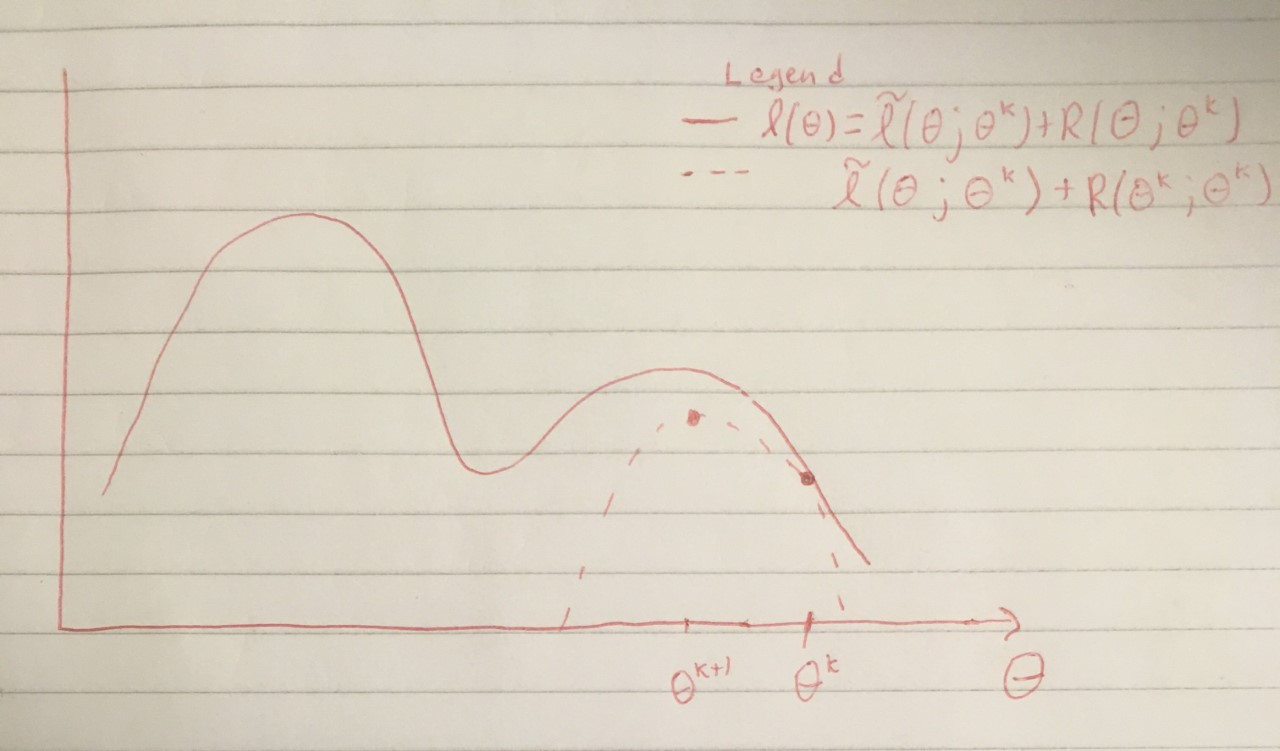
\includegraphics[scale=0.5]{EMv2.png}
% \caption{A visualization of an EM step. In the E-step we compute the dotted curve based on the current values of the parameter $\theta^k$ (up to an additive constant). The dotted curve is guaranteed to lie beneath the log-likelihood and to intersect the log-likelihood curve at $\theta^k$. In the M-step we find a point $\theta^{k+1}$ maximizing the dotted curve. The log-likelihood at $\theta^{k+1}$ is guaranteed to be at least as large as that evaluated at $\theta^k$ because both the value of the dotted curve and the gap between the solid and dotted curve will increase (or at least not decrease).}
% % \end{figure}

% By the above remarks, we see that the EM algorithm is an ascent method; {\bf the likelihood increases at each step}.

